\documentclass[11pt]{article}

\usepackage[margin=1in]{geometry}
\usepackage[T1]{fontenc}
\usepackage{lmodern}
\usepackage{amsmath}
\usepackage{booktabs}
\usepackage{graphicx}
\usepackage{enumitem}
\usepackage{xcolor}
\usepackage[hidelinks]{hyperref}

\setlist{itemsep=2pt, topsep=4pt}
\setlength{\emergencystretch}{2em}
\newcommand{\code}[1]{\texttt{#1}}

\title{Compositional Inconsistency in an Open-Weight Reasoning Model:\\The gpt-oss-120b Pilot on MuSiQue}
\author{William Betts\\[2pt]\small Building on the verification-budget framework of Allison Li}
\date{18 November 2026}

\begin{document}
\maketitle

\begin{abstract}
We ran the pre-registered composition pilot to completion on gpt-oss-120b, an open-weight
reasoning model served by Groq, using the same 100 two-hop MuSiQue questions already scored
for gpt-4.1, gpt-4.1-mini and gpt-5.5. The model answered 37\% of the questions wrongly
(37 of 99; one abstention). Composition disagreement, the total variation distance between
answering a question directly and answering it step by step, predicted these errors with
AUROC 0.68. That is well above stated confidence (0.58) but no better than plain
self-consistency at the same call cost (0.72; difference $-0.03$, 95\% CI $-0.15$ to
$+0.09$). Adding composition to the baseline predictor raised AUROC by $+0.066$, but the
CI includes zero ($-0.022$ to $+0.170$). Under the parent project's fixed verification
budget (25\% of claims checked), self-consistency was the best non-oracle strategy
(reliability 0.835), and composition came in at 0.820. Composition led at the smallest
budgets (6--13\% of claims), and the learned predictor with composition added led at
budgets of 31\% and above. The strongest result is localisation: composition ranked
error-containing regions with AUROC 0.75, the highest of the four models, and 9 of the 10
top-ranked regions held a false claim. Across models, the pattern from the companion paper
holds: on two-hop chains, composition is a real error signal that confidence misses, but
it does not reliably beat self-consistency.
\end{abstract}

\section{Introduction}

The companion paper (\code{paper/paper.tex}, 11 November 2026) tested the composition
signal on three OpenAI models. On 100 two-hop MuSiQue questions, composition was the best
non-oracle strategy under a fixed verification budget for all three models. It added
significant predictive value beyond the baseline only for gpt-4.1-mini, and that gain
disappeared on 300 mixed-length questions. This paper reports the fourth model, the one
the pilot was originally designed for: gpt-oss-120b on Groq's free tier. It ran as a daily
job capped at 200k tokens per day, from 24 October to 18 November 2026.

The question is the same: can a structural signal the model cannot misreport tell a
verifier where to spend a limited checking budget better than the model's own confidence?
For a chain $x \xrightarrow{f} y \xrightarrow{g} z$, a structure-preserving system
satisfies $F(g \circ f)(x) = F(g)(F(f)(x))$, so the composition score
\begin{equation}
  \delta_{\text{comp}} = d_{\mathrm{TV}}\bigl(P_{\text{direct}}(a \mid x),\, P_{\text{stepwise}}(a \mid x)\bigr)
\end{equation}
should be 0 for a model that composes facts consistently. It needs no gold answers.

The gpt-oss run adds three things the OpenAI runs could not:
\begin{itemize}
  \item \textbf{An open-weight model.} The H1 result is no longer specific to one vendor.
  \item \textbf{A reasoning model.} gpt-oss-120b reasons before answering. It ran with
        reasoning effort \code{low} at temperature 0.7. The gpt-5.5 runs needed reasoning
        switched off to accept that temperature.
  \item \textbf{A fourth score on identical questions.} All four models were scored on the
        same 100 audited questions with the same prompts, labels and analysis code. That
        allows direct, paired comparisons across models.
\end{itemize}

\section{Setup}

The protocol is the companion paper's, unchanged. The parts that matter here:
\begin{itemize}
  \item \textbf{Data:} 100 linear two-hop chains from MuSiQue-Ans v1.0 \emph{train}
        (seed 0), all kept after the audit. Open book: every call sees the question's 20
        MuSiQue paragraphs (evidence plus distractors).
  \item \textbf{Model:} \code{openai/gpt-oss-120b} on Groq, temperature 0.7, reasoning
        effort \code{low}, 512 output tokens, one worker.
  \item \textbf{Probes per question:} one original answer with per-step answers and a
        stated confidence (0--100); $N = 3$ direct and $N = 3$ stepwise samples, in two
        independent batches (the same-route control); and $3N = 9$ samples of the original
        question for self-consistency. That comes to about 28 calls per question.
  \item \textbf{Labels:} token F1 $\geq 0.8$ against MuSiQue references counts as correct;
        abstentions are excluded from the primary analysis.
  \item \textbf{H1:} 5-fold out-of-fold logistic regression. The baseline uses confidence,
        hop count, question length, self-consistency and same-route noise; the augmented
        model adds $\delta_{\text{comp}}$. The gain has a 2,000-iteration paired bootstrap
        95\% CI.
  \item \textbf{Fixed budget (Stage F):} each step answer is a claim (200 claims, 55 of
        them false). A strategy checks the top $B$ claims, a caught false claim quarantines
        the later step, and
        $\text{reliability} = 1 - \text{undetected false} / \text{total claims}$. The
        headline $B$ is 25\% of claims, swept from 6\% to 63\%. This stage is not part of
        the daily job, so it was run offline on the cached outputs.
\end{itemize}
The pilot used 2,664 Stage C calls and 6.75M prompt tokens. Free-tier rate limits, not
compute, set the 25-day timeline. Every response is cached, so the analysis reruns for free.

\section{Results}

\subsection{Error prediction (H1)}
Table~\ref{tab:h1} puts gpt-oss-120b next to the three OpenAI models on the same questions.

\begin{table}[h]
\centering
\small
\caption{Single-signal AUROC and H1 gain (95\% CI), pilot100, open book, $N=3$.}
\label{tab:h1}
\begin{tabular}{lrrrrrrl}
\toprule
Model & $n$ & Err. & Conf. & SC & Noise & Comp. & H1 gain \\
\midrule
gpt-oss-120b & 99 & 37\% & 0.58 & \textbf{0.72} & 0.66 & 0.68 & $+0.066$ [$-0.022$, +0.170] \\
gpt-4.1-mini & 96 & 34\% & 0.48 & 0.64 & 0.59 & \textbf{0.67} & $\mathbf{+0.139}$ [+0.035, +0.250] \\
gpt-4.1 & 100 & 30\% & 0.53 & 0.63 & \textbf{0.66} & 0.57 & $-0.026$ [$-0.064$, +0.009] \\
gpt-5.5 & 100 & 34\% & 0.57 & 0.63 & \textbf{0.64} & 0.63 & $+0.001$ [$-0.069$, +0.064] \\
\bottomrule
\end{tabular}
\end{table}

gpt-oss-120b has the highest error rate of the four models but the most readable errors:
every sampling-based signal scores higher on it than on any OpenAI model. Composition
(0.68) is close to its best showing (gpt-4.1-mini, 0.67), but self-consistency is stronger
still. A paired bootstrap puts composition minus self-consistency at $-0.03$ (95\% CI
$-0.15$ to $+0.09$), so the two cannot be told apart at $n = 99$. Composition beats stated
confidence by $+0.10$, but that CI also includes zero ($-0.05$ to $+0.26$).

The H1 gain of $+0.066$ is the second largest of the four models. Its interval overlaps
both gpt-4.1-mini's significant gain and the nulls of the other two models.

\subsection{What the disagreement looks like}
The score is close to binary. Of the 99 scored questions, 48 have $\delta_{\text{comp}} = 0$
(the two routes always agree) and 24 have $\delta_{\text{comp}} = 1$ (they never agree).
That split carries most of the signal:
\begin{itemize}
  \item With $\delta_{\text{comp}} = 0$, 21\% of answers are wrong (10 of 48). These are
        consistently wrong: both routes agree on the same incorrect answer, and no
        consistency check can catch them.
  \item With $\delta_{\text{comp}} > 0$, 53\% are wrong (27 of 51).
  \item 24 questions are inconsistent but correct. Some of this is answer identity: exact
        match after normalisation counts ``May 2, 2008'' and ``May 2'' as different
        answers.
\end{itemize}
The OpenAI models show the same structure (20--23\% error when the routes agree,
39--48\% when they do not). The gap is widest for gpt-oss-120b.

\subsection{Stated confidence}
gpt-oss-120b's confidence is high and flat: 83\% of answers carry a confidence of 90 or
more. Mean confidence is 92.9 on correct answers and 89.3 on wrong ones. That gap is larger
than for the OpenAI models (2.2--3.7 points) but still too small to rank errors well, and
its AUROC is 0.58. This matches the parent project's first research question for a fourth
model: self-reported confidence is a weak guide to which claims to check.

\subsection{Fixed verification budget}
Table~\ref{tab:budget} gives reliability at the headline budget of 50 checks over 200
claims.

\begin{table}[h]
\centering
\small
\caption{Reliability at a 25\% verification budget, pilot100.}
\label{tab:budget}
\begin{tabular}{lrrrrrrr}
\toprule
Model & Random & Dep.-aware & SC & Comp. & Learned & Learned+C & Oracle \\
\midrule
gpt-oss-120b & 0.801 & 0.800 & \textbf{0.835} & 0.820 & 0.825 & 0.830 & 1.000 \\
gpt-4.1-mini & 0.728 & 0.755 & 0.740 & \textbf{0.790} & 0.750 & 0.770 & 0.940 \\
gpt-4.1 & 0.826 & 0.835 & 0.865 & \textbf{0.870} & 0.860 & 0.860 & 1.000 \\
gpt-5.5 & 0.825 & 0.840 & 0.845 & \textbf{0.855} & 0.820 & 0.840 & 1.000 \\
\bottomrule
\end{tabular}
\end{table}

gpt-oss-120b is the first model on which composition is not the best non-oracle strategy at
25\%. Self-consistency catches 22 of the 55 false claims, against 19 for composition.
Composition still beats the parent project's dependency-aware rule ($+0.026$, CI $-0.020$
to $+0.070$), which does no better than random here (0.800 against 0.801), because the
confidence it relies on carries almost no signal.

The ranking depends on the budget (Figure~\ref{fig:budget}):
\begin{itemize}
  \item \textbf{Small budgets (6--13\% of claims):} composition leads, at 0.770 and 0.800
        against 0.750 and 0.770 for self-consistency. With few checks, the questions where
        the routes never agree are the best places to spend them.
  \item \textbf{Middle budgets (19--25\%):} self-consistency ties composition at 19\% and leads at 25\%.
  \item \textbf{Large budgets (31--63\%):} the learned predictor with composition added
        leads, reaching 0.950 at 63\% against 0.945 for composition and 0.925 for
        self-consistency.
\end{itemize}
These sweep points are single evaluations on 100 questions with no confidence intervals.
Treat the crossovers as descriptive, not as findings.

\begin{figure}[h]
\centering
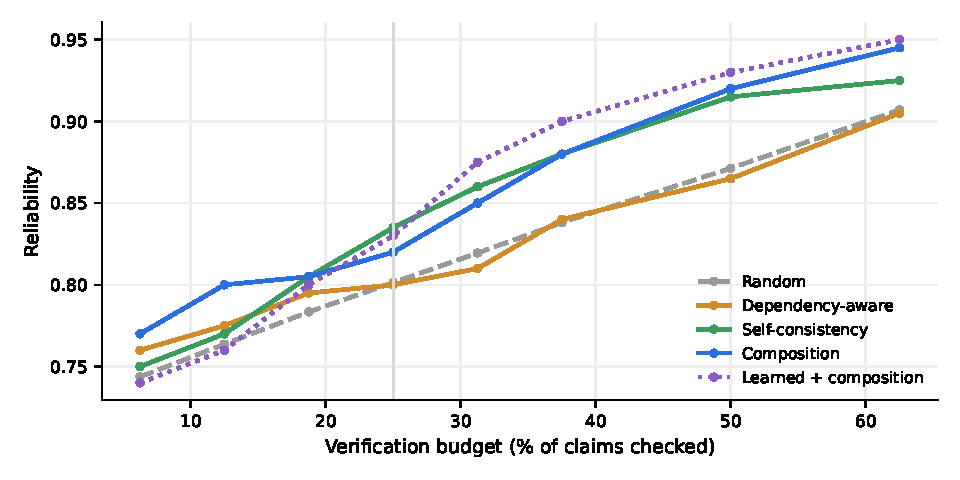
\includegraphics[width=0.85\linewidth]{fig_budget.pdf}
\caption{gpt-oss-120b, pilot100: reliability against verification budget for selected
strategies. The vertical line marks the headline 25\% budget. Oracle (not shown) reaches
1.0 at 25\%.}
\label{fig:budget}
\end{figure}

\subsection{Localisation (H2)}
Composition is better at saying \emph{where} an error is than \emph{whether} the answer is
wrong. It ranks regions that contain a false claim (in either step) above clean ones with
AUROC 0.75, against 0.63--0.68 for the OpenAI models on the same questions. Of the 10
top-ranked regions, 9 contain a false claim, but those 10 cover only 20\% of all false
claims. As in the companion paper, the signal is precise at the top and shallow below.

\subsection{Where the errors come from}
Step 1 (resolving the bridge entity) is wrong in 18\% of questions, and step 2 in 30\%.
A wrong step 1 raises the chance of a wrong final answer only slightly (44\% against 36\%).
That propagation is much weaker than the 0.75 the parent project's PARC-fitted constants
assume. Part of the gap is labelling: token F1 marks ``Knoxville, Tennessee'' against gold
``Knoxville'' as false (F1 0.67), even though the model then answers step 2 correctly.

\subsection{Agreement across models}
The four models largely fail on the same questions. 22 questions are wrong for all four.
gpt-oss-120b shares 24--26 of its 37 errors with each OpenAI model, and 11--13 of its
errors are unique to it. A large shared core of failures points at the questions
themselves, including broken hop renderings, time-sensitive facts and label strictness, as
much as at the models. The planned hand audit should start with these 22.

\section{Discussion and limitations}

Across four models on identical questions, the two-hop picture is now consistent.
\begin{itemize}
  \item \textbf{Confidence is weak everywhere.} Its AUROC ranges from 0.48 to 0.58, and
        the dependency-aware rule built on it is close to random for gpt-oss-120b.
  \item \textbf{Composition is a real signal.} It reaches AUROC 0.57--0.68 for prediction
        and 0.63--0.75 for localisation, and it is best for gpt-oss-120b and gpt-4.1-mini.
  \item \textbf{It does not beat self-consistency.} Under the budget it wins on three of
        four models at 25\% and loses on the fourth. As a predictor it is significant on
        one of four. Self-consistency costs the same number of calls and needs no
        decomposition.
\end{itemize}
The gpt-oss result fits the companion paper's hypothesis that the signal is stronger in
models whose errors come with visible sampling instability. For gpt-oss-120b that
instability is visible to self-consistency too, which absorbs most of composition's
advantage. Where composition keeps an edge is at the top of its ranking: at the smallest
budgets and in localisation.

\paragraph{Limitations.}
\begin{itemize}
  \item \textbf{Two-hop only, $n = 99$.} The CIs are wide: most differences in this paper
        are within noise. The companion paper found that a significant two-hop gain
        disappeared at 300 mixed-length questions.
  \item \textbf{Reasoning effort.} gpt-oss-120b ran with \code{low} reasoning effort, while
        gpt-5.5 had reasoning off. Reasoning and temperature both change the sample
        distributions and are not separated here.
  \item \textbf{Answer identity and labels.} Exact-match identity inflates disagreement
        (24 inconsistent-but-correct questions), and token-F1 labels mark valid
        paraphrases false. Nothing was hand-labelled.
  \item \textbf{Post hoc budget analysis.} Stage F was run after the pre-specified analysis
        and the budget sweep has no intervals.
  \item \textbf{One dataset, train split.} All results are development results.
\end{itemize}

\section{Next steps}

These refine the companion paper's plan for what gpt-oss-120b adds.
\begin{enumerate}
  \item \textbf{Answer-equivalence re-score (no new calls).} Re-score all four pilot100
        runs with a gold-free equivalence judge and check whether the 24
        inconsistent-but-correct gpt-oss questions collapse.
  \item \textbf{Audit the shared failures.} Hand-review the 22 questions all four models
        get wrong and separate model errors from question and label errors.
  \item \textbf{gpt-oss on scale300.} Run the 3- and 4-hop chains with the full-chain
        aggregator pre-registered. The free tier would take months, so this needs a paid
        Groq tier or another gpt-oss host.
  \item \textbf{Composition as a small-budget triage rule.} Pre-register the hypothesis that
        composition beats self-consistency at budgets of 13\% or below, and test it with
        intervals on held-out MuSiQue dev.
  \item \textbf{Reasoning-effort ablation.} Rerun gpt-oss-120b at reasoning efforts
        \code{medium} and \code{high} to check whether more reasoning reduces
        composition failures or just hides them.
\end{enumerate}

\appendix
\section{Reproducibility}

The Groq run lives in \code{will/project1/outputs/}, with every response cached under
\code{cache/groq/}. The comparison runs are in \code{outputs\_openai/runs/}. Nothing below
makes an API call.

\begin{verbatim}
cd will/project1
python3 04_label.py && python3 05_analyze.py   # Stages D-E (the daily job ran these)
python3 06_budget.py                           # Stage F: budget.json, budget_curve.csv
python3 paper_groq/groq_stats.py               # every number in this paper
cd paper_groq && tectonic paper.tex
\end{verbatim}

\code{groq\_stats.py} writes \code{stats.json} (all numbers above, including the paired
bootstraps with seed 0) and \code{fig\_budget.pdf}.

\end{document}
